% Created 2014-04-01 mar 21:25
\documentclass[xcolor={usenames,svgnames,dvipsnames}]{beamer}
\usepackage[utf8]{inputenc}
\usepackage[T1]{fontenc}
\usepackage{fixltx2e}
\usepackage{graphicx}
\usepackage{longtable}
\usepackage{float}
\usepackage{wrapfig}
\usepackage{rotating}
\usepackage[normalem]{ulem}
\usepackage{amsmath}
\usepackage{textcomp}
\usepackage{marvosym}
\usepackage{wasysym}
\usepackage{amssymb}
\usepackage{hyperref}
\tolerance=1000
\usepackage{color}
\usepackage{listings}
\usepackage{gensymb}
\AtBeginSection[]{\begin{frame}[plain]\tableofcontents[currentsection,hideallsubsections]\end{frame}}
\lstset{keywordstyle=\color{blue}, commentstyle=\color{gray!90}, basicstyle=\ttfamily\small, columns=fullflexible, breaklines=true,linewidth=\textwidth, backgroundcolor=\color{gray!23}, basewidth={0.5em,0.4em}, literate={á}{{\'a}}1 {ñ}{{\~n}}1 {é}{{\'e}}1 {ó}{{\'o}}1 {º}{{\textordmasculine}}1}
\usepackage{mathpazo}
\usefonttheme{serif}
\usecolortheme{rose}
\usetheme{Goettingen}
\hypersetup{colorlinks=true, linkcolor=Blue, urlcolor=Blue, breaklinks=true}
\bibliographystyle{plain}
\setbeamercolor{alerted text}{fg=red!50!black} \setbeamerfont{alerted text}{series=\bfseries}
\usetheme{default}
\author{Oscar Perpiñán Lamigueiro (UPM)}
\date{Abril de 2014}
\title{Datos de Radiación Solar}
\hypersetup{
  pdfkeywords={},
  pdfsubject={},
  pdfcreator={Emacs 24.3.1 (Org mode 8.2.1)}}
\begin{document}

\maketitle



\section{Introducción}
\label{sec-1}

\begin{frame}[label=sec-1-1]{Variabilidad Temporal y Espacial}
\begin{itemize}
\item La irradiancia solar extraterrestre depende de la latitud y el instante temporal (\emph{proceso determinista}).
\item La irradiancia solar incidente en la superficie terrestre es resultado de la interacción con la atmósfera cambiante: \alert{variabilidad temporal y espacial} (\emph{proceso estocástico}).
\end{itemize}
\end{frame}
\begin{frame}[label=sec-1-2]{Variabilidad Temporal}
Variabilidad de la irradiación diaria, mensual y anual durante el período comprendido entre 2001-2008 en Carmona, Sevilla
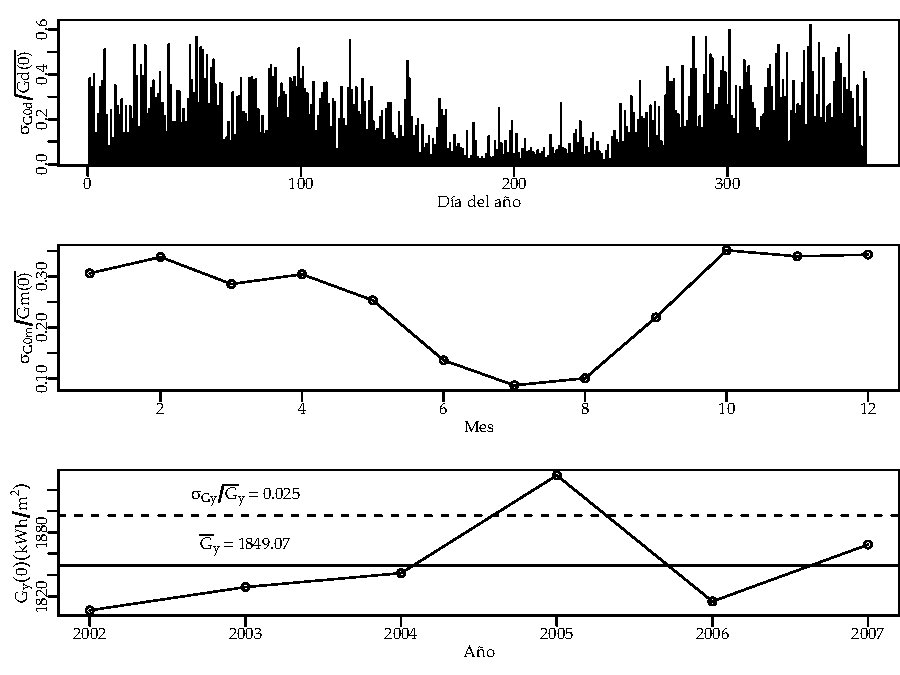
\includegraphics[width=.9\linewidth]{/home/oscar/Copy/Docencia/LibroESF/Figuras/VariabilidadRadiacionDiario.pdf}

\nocite{Perpinan2009}
\end{frame}
\begin{frame}[label=sec-1-3]{Variabilidad Temporal}
\[
\sigma_{\overline{G}}=\frac{\sigma_{G}}{\sqrt{N}}
\]

\begin{itemize}
\item Predicción para un (día, mes, año) \alert{determinado}: 

\begin{itemize}
\item Intervalo de confianza del 95\% acotado por $1.96\cdot\sigma_{G}$
\end{itemize}

\item Predicción para un (día, mes, año) \alert{promedio (durante N años)}: 

\begin{itemize}
\item Intervalo de confianza del 95\% acotado por $1.96\cdot\sigma_{\overline{G}}$
\end{itemize}
\end{itemize}
\end{frame}
\begin{frame}[label=sec-1-4]{Variabilidad Espacial}
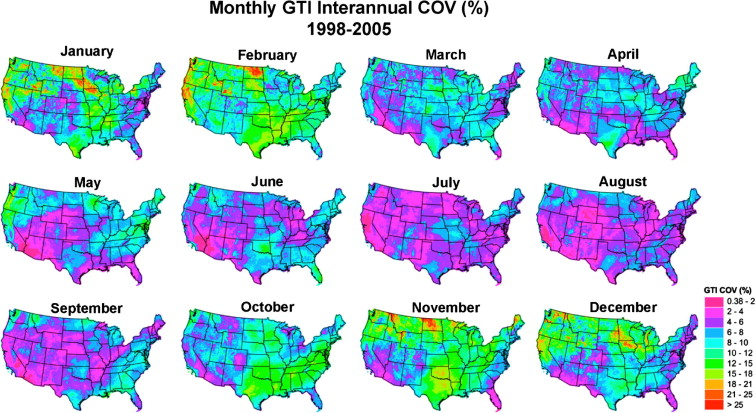
\includegraphics[width=0.9\textwidth]{/home/oscar/Copy/Docencia/LibroESF/Figuras/SpatialVariability.jpg}

\[
COV = 1/G_p \sqrt{\frac{\sum_1^{n}(G_p^2 - G_i^2)}{n}}
\]

\nocite{Gueymard.Wilcox2011a}
\end{frame}
\begin{frame}[label=sec-1-5]{Variabilidad Espacial}
\begin{center}
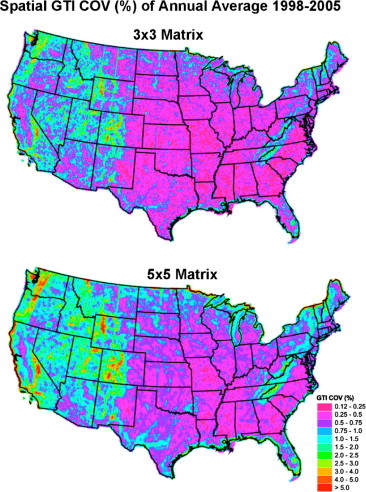
\includegraphics[height=0.9\textheight]{/home/oscar/Copy/Docencia/LibroESF/Figuras/SpatialVariability_Annual.jpg}
\end{center}
\end{frame}
\begin{frame}[label=sec-1-6]{Estimación a partir de Medidas}
\begin{itemize}
\item Para estimar la radiación incidente es necesario contar con:
\begin{itemize}
\item \alert{Medidas cercanas} (variabilidad espacial): distancia no superior a 10 km.
\item \alert{Series temporales} largas (variabilidad temporal): 10 años.
\end{itemize}
\end{itemize}
\end{frame}
\begin{frame}[label=sec-1-7]{Fuentes de datos}
\begin{itemize}
\item \alert{Estaciones meteorológicas}
\begin{itemize}
\item Series largas y con tiempos de muestreo altos.
\item Baja resolución espacial (medidas puntuales)
\item Precisión en caso de medida directa.
\item Tipos: 
\begin{itemize}
\item Con medidor de radiación
\item Sin medidor de radiación (modelos empíricos).
\end{itemize}
\end{itemize}
\end{itemize}

\pause

\begin{itemize}
\item \alert{Imágenes de satélite}

\begin{itemize}
\item Tiempos de muestreo bajos (mejorando)

\item Resolución espacial alta

\item Error debido a la estimación.
\end{itemize}
\end{itemize}

\pause 

\begin{itemize}
\item \alert{Híbrido}

\begin{itemize}
\item Medidas terrestres combinadas con imágenes de satélite
\end{itemize}
\end{itemize}
\end{frame}
\section{Estaciones Meteorológicas}
\label{sec-2}

\begin{frame}[label=sec-2-1]{Estaciones Meteorológicas: medida directa}
\begin{block}{La medida directa de radiación solar se realiza con un piranómetro.}
\end{block}
\begin{columns}
\begin{column}{0.4\textwidth}
\begin{center}
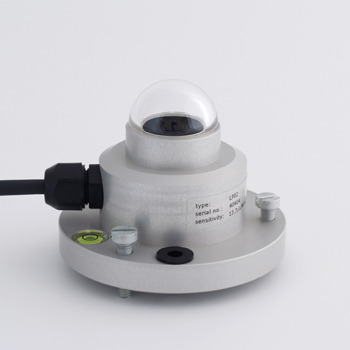
\includegraphics[width=0.8\textwidth]{/home/oscar/Copy/Docencia/LibroESF/Figuras/piranometro.jpg}
\end{center}
\end{column}

\begin{column}{0.6\textwidth}
\begin{itemize}
\item Pila termoeléctrica (termopares con barniz negro)
\item Alojamiento con dos hemiesferas de cristal.
\item Flujo de calor por radiación provoca tensión eléctrica en termopila.
\end{itemize}
\end{column}
\end{columns}
\end{frame}
\begin{frame}[label=sec-2-2]{Estaciones Meteorológicas: medida directa}
\begin{block}{La medida directa de radiación solar se realiza con un piranómetro.}
\end{block}
\begin{columns}
\begin{column}{0.4\textwidth}
\begin{center}
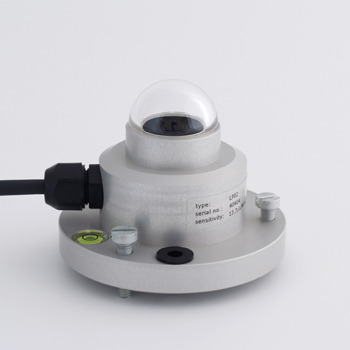
\includegraphics[width=0.8\textwidth]{/home/oscar/Copy/Docencia/LibroESF/Figuras/piranometro.jpg}
\end{center}
\end{column}

\begin{column}{0.6\textwidth}
\begin{itemize}
\item Respuesta espectral plana para radiación visible.
\item Respuesta perfecta al coseno del ángulo de incidencia (pérdidas por reflexión).
\end{itemize}
\end{column}
\end{columns}
\end{frame}
\begin{frame}[label=sec-2-3]{Estaciones Meteorológicas: medida directa}
\begin{block}{La medida directa de radiación solar se realiza con un piranómetro.}
\begin{itemize}
\item Requiere mantenimiento y calibración frecuente.
\end{itemize}
\end{block}
\begin{block}{La red de estaciones que miden directamente radiación es escasa para estimaciones precisas en regiones grandes}
\begin{itemize}
\item La proporción de estaciones con piranómetros es baja respecto a
las que miden temperatura ambiente y precipitación (1:500).
\end{itemize}
\end{block}
\end{frame}
\begin{frame}[label=sec-2-4]{Estaciones Meteorológicas: modelos empíricos}
\begin{block}{Frente a la baja densidad de estaciones con medida directa de radiación se emplean modelos empíricos}
\begin{itemize}
\item Relaciones entre radiación y otras variables
\begin{itemize}
\item Horas de brillo (\emph{sunshine duration})
\item Cobertura nubosa
\item Temperatura ambiente
\item Precipitación
\item Humedad
\item \ldots{}
\end{itemize}
\item Los coeficientes de los modelos sólo se pueden ajustar en estaciones
con medidas de radiación.
\item Los coeficientes dependen del lugar de ajuste, pero se pueden
interpolar para otras localizaciones.
\end{itemize}
\end{block}
\end{frame}
\begin{frame}[label=sec-2-5]{Estaciones Meteorológicas: modelos empíricos}
\begin{itemize}
\item Radiación y Horas de Brillo (Angstrom y Prescott)
\end{itemize}

\[
\frac{G(0)}{B_o(0)} = a_1 + b_1 \frac{S}{S_o}
\]

\begin{itemize}
\item Problema: poca disponibilidad de datos
\end{itemize}
\end{frame}
\begin{frame}[label=sec-2-6]{Estaciones Meteorológicas: modelos empíricos}
\begin{itemize}
\item Radiación y Temperatura (Bristow y Campbell)
\end{itemize}
\[
G(0) = a \left(1 - \exp(-b \Delta T^c)\right) \cdot B_o(0)
\]

\begin{itemize}
\item Variaciones con más variables: Lluvia (si/no), rango antes y después, velocidad viento, humedad relativa.
\end{itemize}

\[
  G(0) = a \left(1 - \exp(-b \Delta T^c)\right) \cdot B_o(0) \cdot \left(1 +
    \sum_1^n p_j \cdot v_j \right) + p_{n+1}
\]

\nocite{Antonanzas-Torres.Sanz-Garcia.ea2013}
\end{frame}
\section{Imágenes de Satélite}
\label{sec-3}

\begin{frame}[label=sec-3-1]{Fundamentos}
\begin{itemize}
\item Los satélites meteorológicos están equipados con \alert{radiómetros}
(sensores de radiación electromagnética a diferentes frecuencias)
que captan \alert{radiación emitida por la Tierra}.

\item La radiación emitida por la Tierra depende de la \alert{reflexión del
suelo}, y la \alert{geometría y composición de la atmósfera}.

\item Diferentes fenómenos físicos se detectan en \alert{bandas de frecuencias}
distintas (canales).

\item Existen diversos procedimientos para \alert{estimar radiación solar} en
superficie a partir de la información de los diferentes canales del
radiómetro.
\end{itemize}
\end{frame}
\begin{frame}[label=sec-3-2]{Satelites Geoestacionarios Europeos: Meteosat}
\begin{itemize}
\item \alert{MFG}: Meteosat First Generation (7 satélites)
\begin{itemize}
\item Equipados con el radiómetro MVIRI (Meteosat Visible and Infrared Imager).
\item Tres canales: visible, infrarrojo, vapor de agua.
\end{itemize}
\item \alert{MSG}: Meteosat Second Generation (3 satélites)
\begin{itemize}
\item Equipados con dos radiómetros:
\begin{itemize}
\item \alert{SEVIRI} (Spinning Enhanced Visible and InfraRed Imager): 12 canales
\item GERB (Geostationary Earth Radiation Budget): infrarrojo visible.
\end{itemize}
\end{itemize}
\end{itemize}

\begin{center}
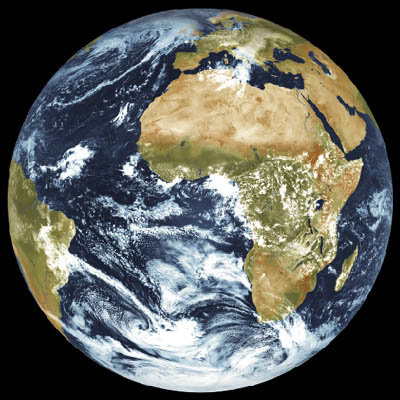
\includegraphics[height=0.3\textwidth]{/home/oscar/Copy/Docencia/LibroESF/Figuras/Tierra_MSG.jpg}
\end{center}
\end{frame}

\begin{frame}[label=sec-3-3]{Procedimientos: Heliosat-2}
\begin{block}{Pasos}
\begin{itemize}
\item Establecer \alert{albedo de referencia} (\emph{suelo}).
\item Estimar \alert{índice de cobertura nubosa}.
\item Estimar radiación en superficie a partir de cobertura nubosa y \alert{modelo de cielo claro}.
\end{itemize}
\end{block}
\begin{block}{}
\begin{itemize}
\item Empleado para base HelioClim
\item Usan datos de MVIRI
\item Accesible via SoDa: \url{http://www.soda-is.com/heliosat/index.html}
\end{itemize}

\nocite{Rigollier.Lefevre.ea2004}
\end{block}
\end{frame}
\begin{frame}[label=sec-3-4]{Procedimientos: CM SAF}
\begin{itemize}
\item \alert{Fundamento}:
\begin{itemize}
\item Se emplea un \alert{Radiative Transfer Model (RTM)}, libRadtran, para
generar una matriz de estados (\alert{Look-up table, LUT}) relaciona la
transmitancia atmosférica y el albedo de la atmósfera para
variedad de estados.
\item La irradiancia en superficie se estima multiplicando la
irradiancia extra-atmosférica por la \alert{transmitancia atmosférica
determinada interpolando en la LUT}.
\end{itemize}
\end{itemize}

\pause

\begin{itemize}
\item \alert{Dos LUTs}: cielo nuboso, cielo claro.
\begin{itemize}
\item \alert{Cielo nuboso}:
\begin{itemize}
\item Estimación de albedo y estado atmosférico a partir de imágenes.
\item Estimación de transmitancia interpolando en LUT para cielo nuboso.
\end{itemize}
\item \alert{Cielo claro}:
\begin{itemize}
\item Estimación de transmitancia interpolando en LUT para cielo claro \alert{sin estimación previa} de albedo.
\end{itemize}
\end{itemize}
\end{itemize}

\pause

\begin{itemize}
\item Emplean datos del \alert{radiómetro MSG/SEVIRI}
\end{itemize}

\nocite{Mueller.Matsoukas.ea2009}
\end{frame}


\begin{frame}[label=sec-3-5]{Procedimientos: LSA SAF}
\begin{itemize}
\item Generación de \alert{máscara de nubes} a partir de imagen usando algoritmo de \href{http://www.nwcsaf.org/}{NWC-SAF}.
\item Para \alert{zonas sin nubes}: modelo de cielo claro sin usar datos de imagen.
\item Para \alert{zonas cubiertas}: modelo de transmitancia atmosférica a partir de imágenes.
\item Emplean datos del \alert{radiómetro MSG/SEVIRI}
\end{itemize}

\nocite{Geiger.Meurey.ea2008}
\end{frame}
\section{Fuentes de Datos: Estaciones Terrestres}
\label{sec-4}

\begin{frame}[label=sec-4-1]{Baseline Surface Radiation Network}
\begin{block}{\url{http://www.bsrn.awi.de/}}
\begin{itemize}
\item BSRN provides near-continuous, long-term, in situ-observed,
Earth-surface, broadband irradiances (solar and thermal infrared)
and certain related parameters from a network of more than 50
globally diverse sites.
\end{itemize}

\begin{center}
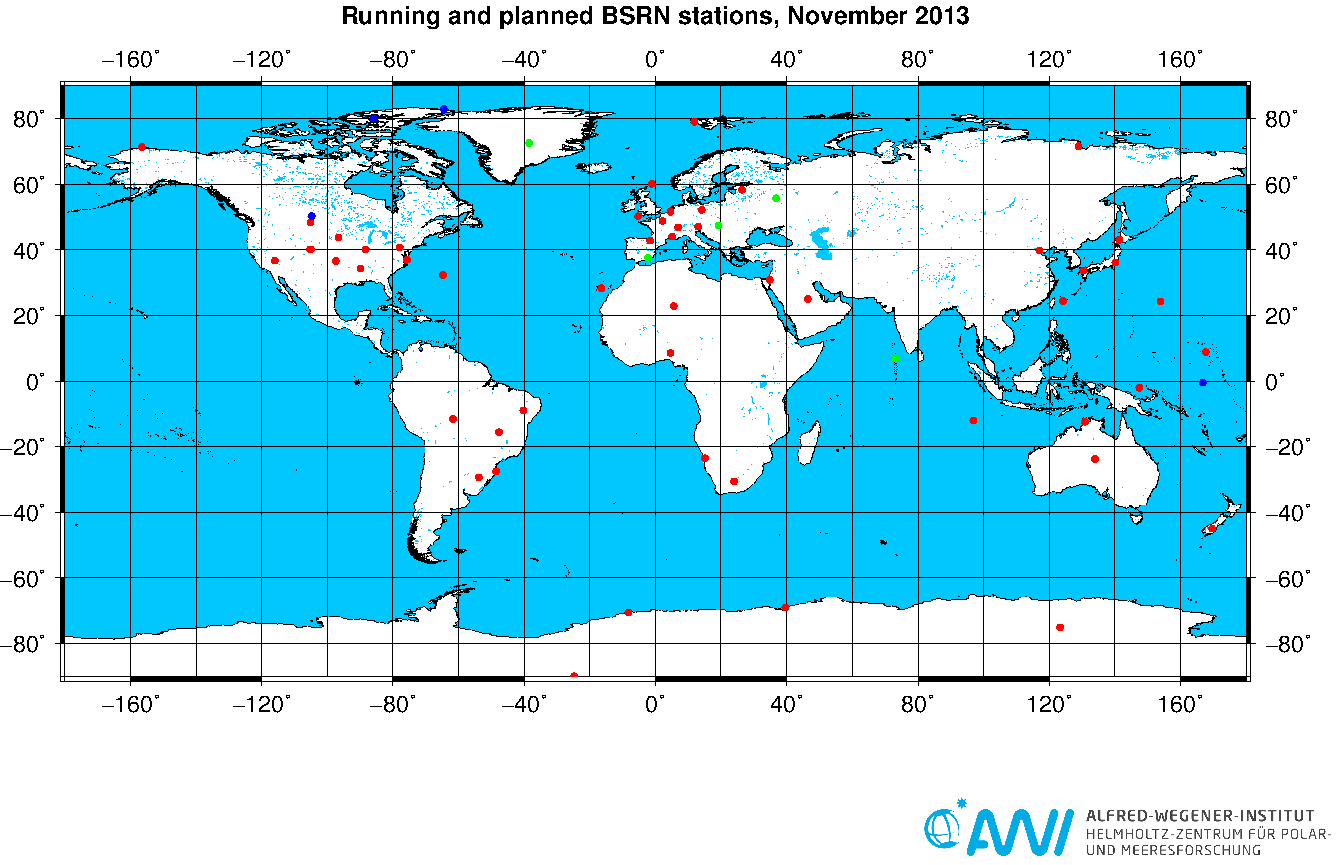
\includegraphics[height=0.5\textheight]{/home/oscar/Copy/Docencia/LibroESF/Figuras/BSRN.png}
\end{center}
\end{block}
\end{frame}
\begin{frame}[label=sec-4-2]{Baseline Surface Radiation Network}
\begin{itemize}
\item Validation and confirmation of satellite and computer model
estimates.

\item Datos desde:  \url{http://www.bsrn.awi.de/en/data/data_retrieval_via_pangaea/}
\end{itemize}
\end{frame}

\begin{frame}[label=sec-4-3]{Measurement and Instrumentation Data Center NREL}
\begin{block}{\url{http://www.nrel.gov/midc/}}
Radiación global, directa y difusa (y otras variables) con muestreo de
  1 min en diversas localidades de EEUU.

\begin{center}
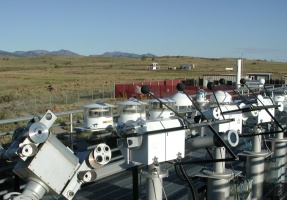
\includegraphics[height=0.3\textheight]{/home/oscar/Copy/Docencia/LibroESF/Figuras/NRELStation.jpg}
\end{center}
\end{block}
\end{frame}
\begin{frame}[label=sec-4-4]{MAGRAMA-SIAR}
\begin{block}{\url{http://eportal.magrama.gob.es/websiar/Inicio.aspx}}
\begin{itemize}
\item El Sistema de Información Agroclimática para el Regadío (SiAR)
registra datos agroclimáticos relacionados con demanda hídrica de
las zonas de riego.

\item Más de 400 estaciones.

\item Valores diarios y horarios
\end{itemize}

\begin{center}
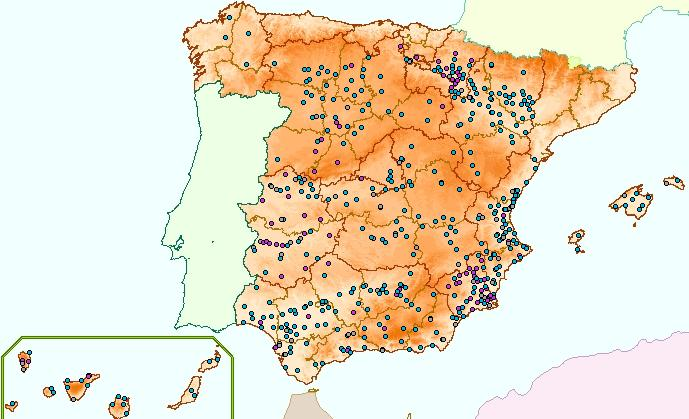
\includegraphics[height=0.35\textheight]{/home/oscar/Copy/Docencia/LibroESF/Figuras/EstacionesSIAR.jpeg}
\end{center}
\end{block}
\end{frame}
\begin{frame}[label=sec-4-5]{MAGRAMA-SIAR}
\begin{block}{Sensores}
\begin{itemize}
\item Temperatura y Humedad
\item Piranómetro
\item Anemoveleta
\item Pluviómetro
\item Temperatura del suelo  (algunas)
\end{itemize}

\begin{center}
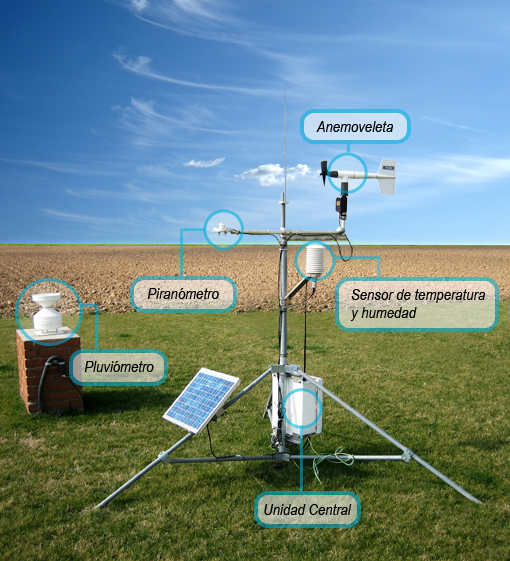
\includegraphics[height=0.4\textheight]{/home/oscar/Copy/Docencia/LibroESF/Figuras/EstacionSIAR.png}
\end{center}
\end{block}
\end{frame}

\begin{frame}[label=sec-4-6]{AEMET}
\begin{block}{\href{http://www.aemet.es/es/eltiempo/observacion/radiacion}{Radiación}}
\begin{itemize}
\item Alrededor de 30 estaciones en todo el territorio.
\item Medidas de global, difusa y directa.
\item Sólo gráficas.
\end{itemize}
\end{block}
\begin{block}{\href{http://www.aemet.es/es/eltiempo/observacion/ultimosdatos}{Estaciones \guillemotleft{}convencionales\guillemotright{}}}
\begin{itemize}
\item Presión, temperatura, viento, humedad, lluvia.
\item Permite descarga de datos horarios por día.
\end{itemize}
\end{block}
\end{frame}
\begin{frame}[label=sec-4-7]{Redes de Comunidades Autónomas}
\begin{itemize}
\item \href{http://www2.meteogalicia.es/galego/observacion/estacions/estacions.asp}{Meteogalicia}
\item \href{http://meteo.navarra.es/estaciones/mapadeestaciones.cfm}{MeteoNavarra}
\item \href{http://www.meteo.cat/xema/AppJava/SeleccioPerComarca.do}{Cataluña}
\end{itemize}
\end{frame}
\section{Fuentes de Datos: Satélite}
\label{sec-5}

\begin{frame}[label=sec-5-1]{SSE-NASA}
\begin{block}{Surface meteorology and Solar Energy (SSE)}
\begin{itemize}
\item 200 satellite-derived meteorology and solar energy parameters
  \alert{monthly averaged} from 22 years of data
\item Resolución 1ºx1º
\end{itemize}

\url{https://eosweb.larc.nasa.gov/cgi-bin/sse/sse.cgi}
\end{block}
\end{frame}
\begin{frame}[label=sec-5-2]{EUMETSAT - SAF}
\begin{itemize}
\item \alert{\href{http://www.eumetsat.int}{EUMETSAT}} is the European operational satellite agency for monitoring
weather, climate and the environment.
\item \alert{\href{http://www.eumetsat.int/website/home/Satellites/GroundSegment/Safs/index.html}{Satellite Application Facilities} (SAFs)}
\begin{itemize}
\item Dedicated centres of excellence for processing satellite data.
\item Generate and disseminate operational EUMETSAT products and
services.
\end{itemize}
\end{itemize}
\end{frame}
\begin{frame}[label=sec-5-3]{SAFs}
\begin{itemize}
\item \href{http://www.cmsaf.eu/bvbw/appmanager/bvbw/cmsafInternet}{SAF on Climate Monitoring (CM SAF)}: provision of satellite-derived geophysical parameter data sets suitable for \alert{climate monitoring}

\begin{itemize}
\item Environmental Data Records (EDR): time-tagged earth-located
geophysical parameters produced from sensor data. EDRs are derived
in low to medium latency not fulfilling strictest climate
requirements.

\item Climate Data Records (CDR): time series of measurements of
sufficient length, consistency, and continuity to determine climate
variability and change.
\end{itemize}

\item \href{http://landsaf.meteo.pt}{SAF on Land Surface Analysis} (LSA SAF): generates, archives and
disseminates, on an \alert{operational basis}, a set of parameters involved
in the surface radiation budget, evapotranspiration, vegetation
cover and and fire-related products.
\end{itemize}
\end{frame}
\begin{frame}[label=sec-5-4]{SAFs: Radiación}
\begin{itemize}
\item \alert{CM SAF}: Surface incoming shortwave radiation (\href{http://wui.cmsaf.eu/safira/action/viewDoiDetails?acronym=RAD_MVIRI_V001}{SIS})

\begin{itemize}
\item AEMET ha analizado las estimaciones para España en su \href{http://www.aemet.es/es/serviciosclimaticos/datosclimatologicos/atlas_radiacion_solar}{Atlas de Radiación}.
\end{itemize}

\item \alert{LSA SAF}: Down-welling surface short-wave radiation flux (\href{http://landsaf.meteo.pt/algorithms.jsp?seltab=1&starttab=1}{DSSF})
\end{itemize}
\end{frame}
\begin{frame}[label=sec-5-5]{ADRASE - CIEMAT}
\begin{block}{\url{http://adrase.es}}
\begin{itemize}
\item Radiación solar media mensual, resolución aproximada de 5x5 km.
\begin{itemize}
\item Media mensual y anual más probable durante un periodo de largo
plazo (imágenes de satélite, modelo aproximadamente Heliosat)
\item Variabilidad esperada de los valores diarios mensuales: (series
largas de datos de estaciones de AEMET y extrapolación espacial
con IDW)
\end{itemize}
\end{itemize}

\begin{center}
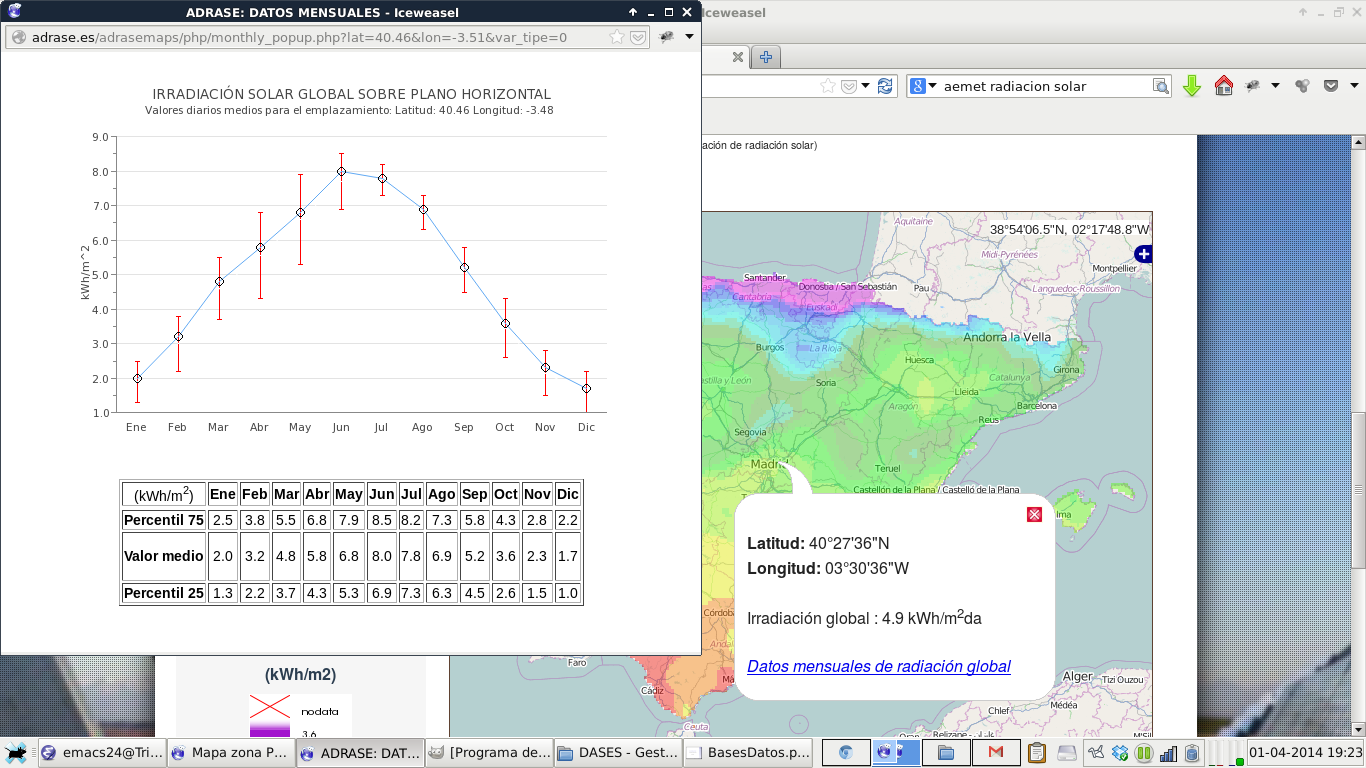
\includegraphics[height=0.35\textheight]{/home/oscar/Copy/Docencia/LibroESF/Figuras/adrase.png}
\end{center}
\end{block}
\end{frame}
\section{Métodos híbridos}
\label{sec-6}

\begin{frame}[label=sec-6-1]{Interpolación Espacial}
\begin{block}{\alert{Objetivo}: mejorar la resolución espacial de medidas dispersas}
\begin{itemize}
\item \alert{Inverse Distance Weighting (IDW)}: determinista.

\item \alert{Ordinary Kriging}: modelo determinista para la media (constante) y estocástico para residuos.
\end{itemize}

\[
  \hat{z}(\mathbf{s}) = \mu + \epsilon(\mathbf{s})
\]

\begin{itemize}
\item \alert{Kriging with External Drift (KED)}: modelo determinista para la media incorporando información de una variable con alta densidad espacial.
\end{itemize}
\[  \hat{z}(\mathbf{s}_\theta) =  \sum_{k=0}^p \hat{\beta}_k q_k(\mathbf{s}_\theta) + 
  \sum_{i=1}^n \lambda_i \epsilon(\mathbf{s}_i)
\]

\nocite{Journee.Bertrand2010}
\nocite{Antonanzas-Torres.Canizares.ea2013}
\nocite{Bojanowski.Vrieling.ea2013}
\end{block}
\end{frame}

\begin{frame}[label=sec-6-2]{Corrección por topografía}
\begin{block}{Sky-View Factor (SVF)}
Proporción de cielo visible para un receptor horizontal (afecta a la radiación difusa isotrópica)
\[
SVF=1-\int_0^{2\pi}sin^{2} \theta_{hor} d\theta
\]
\end{block}
\begin{block}{Horizon blocking}
Bloqueo de región circunsolar por horizonte: afecta a radiación
directa y difusa anisotrópica
\end{block}
\end{frame}
\begin{frame}[label=sec-6-3]{Corrección por topografía}
\begin{center}
\includegraphics[height=0.9\textheight]{/home/oscar/R/downscaling/paper/algorithmScheme.pdf}
\end{center}
\end{frame}

\begin{frame}[label=sec-6-4]{Corrección por topografía}
\begin{center}
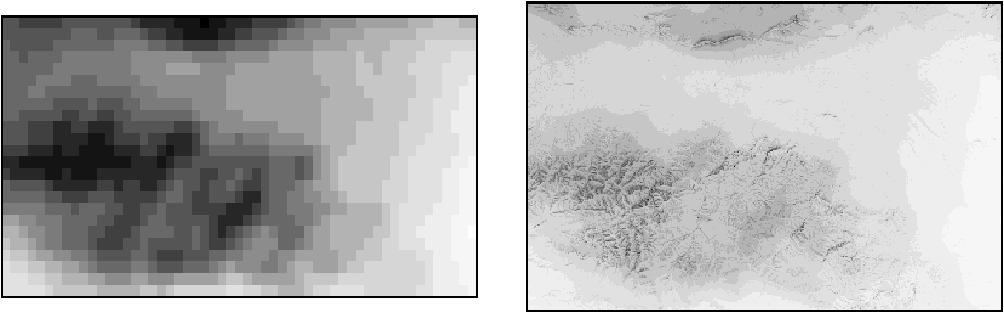
\includegraphics[width=0.9\textwidth]{/home/oscar/Copy/Docencia/LibroESF/Figuras/downscaling.pdf}
\end{center}

\nocite{Bosch.Batlles.ea2010}
\nocite{Tovar-Pescador.Pozo-Vazquez.ea2006}
\nocite{Antonanzas-Torres.MartinezdePison.ea2013}
\nocite{Hofierka.Suri2002}
\end{frame}
\begin{frame}[fragile,label=sec-6-5]{PVGIS - \texttt{r.sun}}
 \begin{block}{\url{http://re.jrc.ec.europa.eu/pvgis/apps4/pvest.php}}
PVGIS (Photovoltaic Geographical Information System) is a research,
demonstration and policy-support instrument for geographical
assessment of the solar energy resource in the context of integrated
management of distributed energy generation.
\begin{itemize}
\item Computation of clear-sky global irradiation on a horizontal surface
\item Sky obstruction by local terrain features (hills or mountains)
calculated from the digital elevation model.
\item Interpolation of the clear-sky index and computation of global
irradiation on a horizontal surface.
\end{itemize}
\end{block}
\end{frame}

\section{Bibliografía}
\label{sec-7}

\begin{frame}[allowframebreaks,label=]{Bibliografía}
\bibliography{/home/oscar/Dropbox/bibliografia/BibUTF8}
\end{frame}
% Emacs 24.3.1 (Org mode 8.2.1)
\end{document}